\documentclass{apnet18}

\usepackage{times}
\usepackage{epsfig}
\usepackage[TABBOTCAP]{subfigure}
\usepackage{tabularx}
\usepackage{graphicx}
\usepackage{color}
\usepackage{xspace}
\usepackage{thumbpdf}
\usepackage{listings}
\usepackage{verbatim}
\usepackage{hyperref}
\usepackage{booktabs}
\usepackage{colortbl}

\usepackage{colortbl,booktabs}%
\usepackage{subfigure}
\usepackage{amsmath}
\usepackage{algorithm}    
\usepackage{algorithmic} 



\hypersetup{pdfstartview=FitH,pdfpagelayout=SinglePage}

\setlength\paperheight {11in}
\setlength\paperwidth {8.5in}
\setlength{\textwidth}{7in}
\setlength{\textheight}{9.25in}
\setlength{\oddsidemargin}{-.25in}
\setlength{\evensidemargin}{-.25in}
%\setlength{\headsep}{0in}
%\pagenumbering{arabic}


\renewcommand\thesection{\arabic{section}} 

\newcommand{\eg}{{\it e.g.,}\xspace}
\newcommand{\ie}{{\it i.e.,}\xspace}
\newcommand{\fillme}{{\bf XXX}~}
\newcommand{\jc}[1]{{\footnotesize\color{blue}{[JC: #1]}}} %[JC: #1]}}}


%\newcommand{\comment}[1]{}

\newenvironment{packeditemize}{\begin{list}{$\bullet$}{\setlength{\itemsep}{0.5pt}\addtolength{\labelwidth}{-4pt}\setlength{\leftmargin}{\labelwidth}\setlength{\listparindent}{\parindent}\setlength{\parsep}{1pt}\setlength{\topsep}{0pt}}}{\end{list}}

\begin{document}

\conferenceinfo{APNet 2018} {}
\CopyrightYear{2018}
\crdata{X}
\date{}

%%%%%%%%%%%% THIS IS WHERE WE PUT IN THE TITLE AND AUTHORS %%%%%%%%%%%%

\title{Dante: An FOV-Aware FEC-Based Protocol for 360-Degree Video Streaming}

\maketitle

%\thispagestyle{empty}


	
%%%%%%%%%%%%%  ABSTRACT GOES HERE %%%%%%%%%%%%%%
\section*{Abstract}
As 360-degree videos grow dramatically in popularity, more 
applications demand the ability to stream 360-degree videos to 
wirelessly connected devices, such as smartphone headsets. However, 
the limited and unstable network capacity of wireless networks make 
them ill-suited to the quality of experience requirements of 
360-degree videos, \ie high resolution with low delay and little 
jitter. A natural solution is to leverage the fact that at any 
moment, a viewer watches only a small spatial region of the video, 
called FOV (field of view), which allows for better allocation of 
network bandwidth in the region that the user actually watches. 
Previous efforts on 360-degree videos have largely focused on how to 
differentiate spatial areas by different encoded bitrates. While we 
also use the concept of FOV-aware streaming, this paper explores a 
different design space than application-layer adaptation. We present 
a custom UDP-based transport strategy, called {\em Dante}, which 
adapts to dynamic network conditions by encoding and scheduling data 
packets based on how close they are to the FOV. Dante is 
complementary to application-level bitrate adaptation strategies, and
can be deployed by replacing the existing underlying transport 
protocol with minimal changes to the video player. Experimental 
results show that Dante achieves 20\% to 30\% 360-degree video PSNR performance gain compared to traditional video transport schemes.

%360-degree videos have been widely applied due to its unprecedented immersive experience. The appreciation of watching 360-degree videos
%on untethered mobile devices, such as smartphone headsets,
%is considered to be a more promising trend, which, however, is hampered by the
%poor Quality of Experience (QoE), subject to limited bandwidth and error-prone characteristic of wireless networks.
%Fortunately, the key observation that only a small portion of a 360-degree video is
%perceived by users at any time, i.e., Field Of View (FOV), implies that unequal attention
%should be given different regions spatially and can
%be utilized to mitigate dependence on stable network condition and ultra-high bandwidth. Currently, the state-of-the-art schemes, like FOV-aware tile-based streaming in the application layer, almost based on FOV-aware bit-rate adaptation, transport protocol of which, however, fails to consider FOV. So, we propose an application-layer protocol, reliability scheme of which is FOV-aware and performs hierarchical protection to boost QoE of 360-degree videos in mobile scenarios. Experiments demonstrate our protocol achieves desirable improvements over the reference schemes in QoE of 360-degree videos.

\section{Introduction}

% 360 degree videos are important
360-degree videos are coming to age, which has been driven by content
providers (\eg CNN, New York Times) serving more immersive content (\eg 
NBC broadcasting the 2018 Winter Olympics in VR~\cite{NBC_olympic_360}), as well as 
by more application platforms~\cite{google_developers,facebook360} and 
devices (\eg Samsung smartphone headset~\cite{SUMSUNG_HEADSET}).
However, streaming 360-degree videos to mobile devices through wireless
networks remains a substantial challenge.

% why it's challenging
To provide true immersive experience, the 360-degree video must be streamed
in high resolution and within a small bounded delay.

\begin{packeditemize}
% low delay
\item {\em Stringent delay constraint:} 

To prevent simulator sickness \cite{Simulator_Sickness} and to provide good Quality of Experience (QoE), the vendors of HeadMounted Displays (HMD) recommend that the video systems
react to head movements as fast as the HMD refresh rate, i.e., frames per second (fps).
Since fps of state-of-the-art HMDs is 120 Hz,
the whole system should react in less than 10 ms. These stringent delay constraints render many traditional streaming 
protocols (\eg~\cite{MPEG-DASH},~\cite{FESTIVE}) insufficient.

%\jc{reword the last sentence. what's "application round-trip latency"? why "sickness" is caused by some "refresh rate"?} These stringent delay constraints render many traditional streaming  protocols (\eg~\cite{??,??}) insufficient.

% high bandwidth
\item {\em High-bandwidth consumption:}
Moreover, 360-degree videos require high bandwidth to stream videos in
high resolution, ideally, over the whole 360-degree sphere; \eg the 
bitrate of an 8K 360-degree video feed encoded at a frame rate of 60 fps
(frames per second) with HEVC~\cite{HEVC} is $\sim$100Mbps. According to
OpenSignal~\cite{opensignal}, almost a half of the 77 surveyed 
countries in 2017 over the world only have access to 4G cellular 
networks of 10-25 Mbps.
\end{packeditemize}

% fov-aware streaming & problems
One of the common approaches to addressing this challenge is that, 
instead of streaming all video content simultaneously, one can stream
only the video content in and around the viewer's field of view (FOV),
or prioritize data in those FOV regions over non-FOV regions. This 
FOV-aware approach has attracted great attention in recent 
years~\cite{Viewport-adaptive,360ProbDASH,Adaptive_Streaming_Framework,Two-tier,Omnidirectional_Video_over_HTTP,Furion}, 
leading to many strategies that adapt application-level parameters, \eg 
encoding bitrate, to allocate bandwidth so as to ensure good quality of
content in the FOV regions. However, these application-level strategies 
do not directly optimize for the delay constraints. This is because 
they run on top of existing transport protocols that are unaware of FOVs
and thus fail to leverage the fact that data packets may have different
inherent priority depending on whether the carried video data belong to
FOV region.

% custom transport protocols & problems
On the other hand, there have been proposals of custom transport 
protocols for streaming delay-sensitive videos~\cite{MPMTP,CMT-VR,ADMIT}. 
Unfortunately, they have so far focused on traditional video content, 
as opposed to 360-degree videos. So the opportunities of developing a 
custom transport protocol for 360-degree video streaming remain untapped.
In particular, it remains unclear how to leverage the knowledge of FOV
to adapt transport-level actions, \eg packet scheduling and setting of 
the redundancy level in error correction code.

% our solution
In this paper, we propose {\em Dante}, an FOV-aware transport protocol
for 360-degree video streaming. Figure. 2 puts Dante into the perspective
of previous efforts. At the core of Dante are two ideas. First, like 
other video-specific custom streaming protocols, Dante does not enforce
total reliability which are likely to be blocked by re-transmissions, 
Dante uses Forward Error Correction (FEC) to recover data losses 
without retransmissions, thus significantly reducing the streaming delay.
While these protocols might cause small fraction of missing frames 
(except key frames for which we do apply retransmission to ensure 
reliability), our evaluation shows that its impact on video quality is 
negligible, even under highly lossy network connections. 
Second, Dante prioritizes FOV regions by using more FEC redundancy to 
send data packets belonging to FOV regions (predicted by the 
video player). This effectively gives packets in FOV regions more 
bandwidth, higher reliability, and more chance to meet the streaming 
delay constraint.

We use two video sequences downloaded from Youtube as our dataset to evaluate the performance of Dante. The experimental results show that Dante improves video PSNR over current video transport protocols by 20\% to 30\%.

%\jc{need a para to summarize the key results: 
%we use what dataset to evaluate the performance of Dante and compares it against what baseline.  the experimental results show that Dante improves what metrics over  what baselines by how much}













%%% OLD INTRO
\begin{comment}
	
With the promise of immersive visual experience, 360-degree videos are widely applied in sports field, social field~\cite{facebook360}, and apps development field~\cite{google_developers}, etc. Meanwhile, it has been well deployed across mainstream content providers such as NBC (who broadcast the 2018 winter Olympics in VR), news outlets, such as CNN, New York Times, and user-generated content platform such as Youtube and Facebooks.
However, some significant challenges still remain as the major bottlenecks for 360-degree technologies, even worse in mobile scenarios.

The bottleneck can be summarized as that wireless links are characterized by limited resources and error-prone problems, while 360-degree video streaming
is characterized by bandwidth intensiveness and delay sensitivity.

%% One aspect of technological challenges stems from stringent delay and high bandwidth requirement. 
%% To prevent simulator sickness~\cite{Simulator_Sickness}, the whole system needs to react as fast as the refresh rate of Head-mounted Display(HMD), such as 120 Hz, in other words, this means application round-trip latency is supposed to be less than 10ms for imperceptible Motion-To-Photon(MTP) latency. Such the rigorous delay constraint prevents the implementation of those traditional protocols based on feedback and retransmissions.
For example, application round-trip latency is supposed to be less than 10ms for imperceptible Motion-To-Photon(MTP) latency in order to prevent simulator sickness~\cite{Simulator_Sickness}, due to the refresh rate of Head-mounted Display(HMD), such as 120 Hz. Such the rigorous delay constraint prevents the implementation of those traditional protocols based on feedback and retransmissions.

Meanwhile, 360-degree videos have the requirement of high bandwidth in order to enable immersive experience. The bit-rate of 8K 360-degree videos at 60 fps encoded using High Efficiency Video Coding (HEVC)~\cite{HEVC} is around 100 Mbps. However, according to OpenSignal~\cite{opensignal}, covering 77 countries in the world, almost a half of countries have access to 4G cellular network with only 10-25 Mbps speed in 2017. Obviously, it's not available and practical to deploy 360-degree videos service in mobile scenarios.    

Currently, based on the observation that only the FOV region of video is only perceived by user anytime, FOV-aware tile-based streaming~\cite{Viewport-adaptive}\cite{360ProbDASH}\cite{Adaptive_Streaming_Framework} \cite{Two-tier}\cite{Omnidirectional_Video_over_HTTP}\cite{Furion}, a scheme of application layer, is proposed to mitigate the requirement of bandwidth and delay, due to the introduction of FOV-aware bit-rate adaptation and video segment prefeatching. However, it achieves poor performance over wireless links, featured by limited bandwidth and error-prone characteristic, because the most advanced transport protocols it uses fail to consider FOV, for example, their reliability schemes of transport layer fail to consider FOV.     

In this paper, we propose Dante, as depicted in Figure 1, an application-layer 360-degree video protocol.
In this proposed Dante, instead of only transmissions, FEC is adopted to strengthen reliability scheme, which can recover data loss over wireless lossy links, mitigating video quality degradation. 
And the core of the reliability scheme is an FEC adaptation, which is FOV-aware and performs hierarchical error protection on different region of the video, spatially.

%We first design a FOV-aware video distortion model, and from the perspective of reliability schemes, design an FOV-aware FEC parameter adjusting algorithm based on that model to achieve low latency. Furthermore, we design an FOV-aware packet scheduling algorithm, which preferentially allocates better bandwidth for more crucial data, and thus boosting video quality and achieving graceful degradation even under poor network condition.
\end{comment}

\begin{figure}[ht]
	\centering
	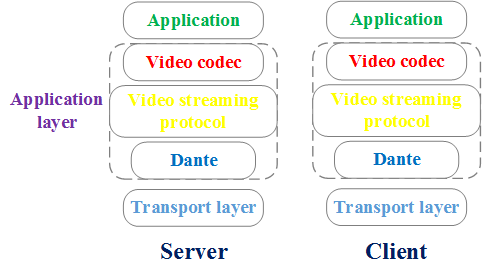
\includegraphics[scale=0.4]{paper_figs/stack_dante.png}
	\caption{Illustration Of Dante}
	\label{paper_figs:pathdemo}
\end{figure}

\begin{figure}[ht]
	\centering
	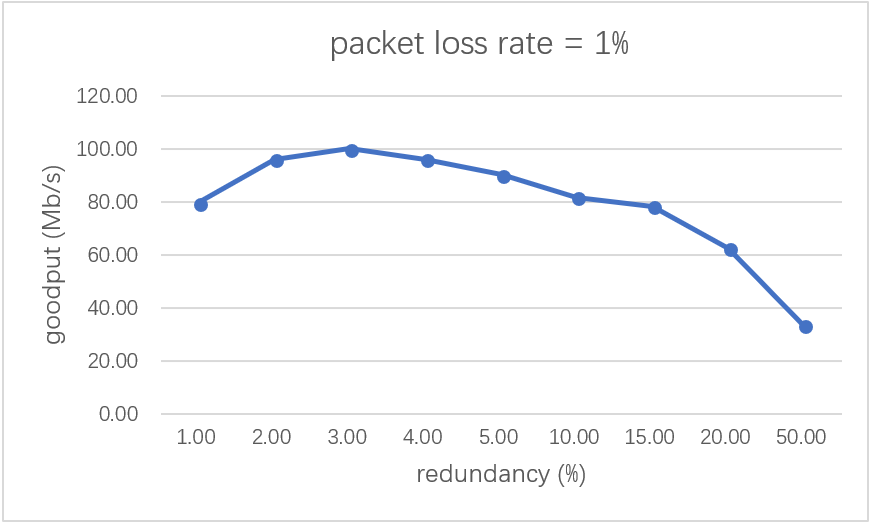
\includegraphics[scale=0.25]{paper_figs/tradeoff_only_goodput.png}
	\caption{The Goodput When Increasing The FEC Redundancy}
	\label{paper_figs:pathdemo}
\end{figure}



\section{Background And Motivation}

	Generally, VR headset has a 110 degree horizontal FOV and a 90 degree vertical FOV, and the fraction of videos of video which extracted and displayed on HMD anytime would be $\frac{{110^\circ }}{{360^\circ }} \times \frac{{90^\circ }}{{180^\circ }}{\rm{ = }}15{\rm{\% }}$. Obvious, the data of the FOV region, viewed by users, is more important than non-FOV region.
	From the perspective of application layer, the FOV-aware tile-based streaming schemes, based on Dynamic Adaptive Streaming over HTTP (DASH), suggests that, 360-degree videos are split and encoded into multiple tiles spatially, each of which can be independently decoded, stored into a single file. Furthermore, according to the distance from the expected viewpoint of users, 360 videos would be split into two or three regions spatially, each of which would be composed of multiple contiguous tiles and store into a single file, as depicted in Figure 3.
	
	\begin{figure}[ht]
		\centering
		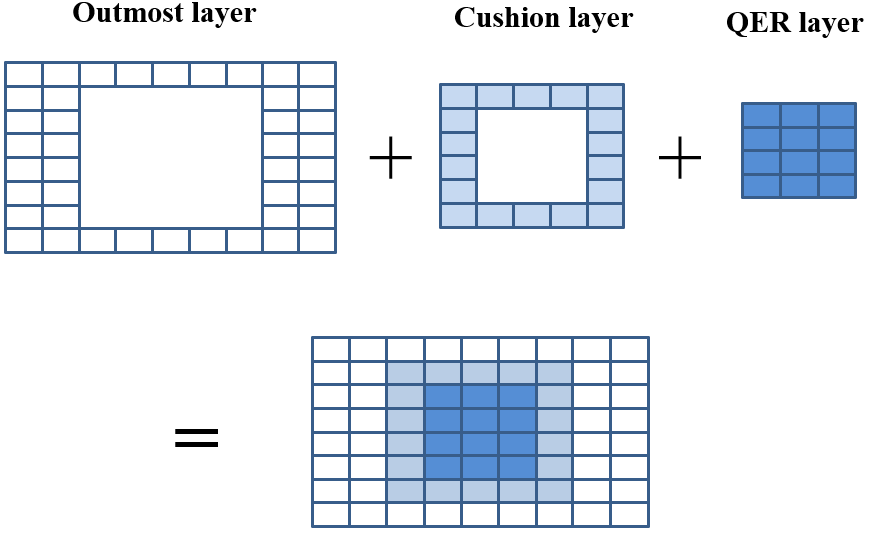
\includegraphics[scale=0.2]{paper_figs/tileSplit.png}
		\caption{360-degree Video Representation}
		\label{paper_figs:pathdemo}
	\end{figure}	
	
	
	However, the state-of-the-art transport schemes, which are not FOV-aware, spend as same amount of bandwidth on reliable delivery of trivial data, i.e., the non-FOV data, as the FOV data. So, can we, from the perspective of reliability of transport, design a protocol, which prioritizes the reliability of FOV data over non-FOV data, boosting the whole system performance by sacrificing little degree of quality of non-FOV data.

    
	Instead of only retransmissions, FEC\footnote{In Dante, FEC is generated through erasure coding of blocks of packets, to recover lost packets, which should be distinguished from FEC, computed on individual packets using channel coding, recovers from bit errors.} is adopted to be a proactive scheme of reliability in our proposed protocol. It can achieve low delay by mitigating retransmissions and is generally be in favoured by real-time video services. However, how to adjust the degree of FEC redundancy is a challenging problem. 
	 
	For example, considering a chunk of data organized into K packets, with equal length, the FEC encoder takes the K data packets, and adds A repair packets to create a coded block of size ${\rm{B = (K + A)}}$. The receiver can recover completely the origin data of $K$ packets if any not less than $K$ packets of all ${K + A}$ packets are received. The code rate is equal to ${K/B}$ and the redundancy of FEC is ${(A/K)}$ . Obviously, it can recover $A$ packets of loss over lossy links at most and when FEC redundancy packets is more, the coding system has more powerful recoverability. 	 
	
    Increasing FEC redundancy can improve recovery probability of data packets in order to mitigate the degradation of video quality caused by packet transmission loss. However, with the increasing of redundancy and computing overhead of coding \cite{ASCOT}, the over-provisioning of redundancy may enlarge end-to-end delay, even causing unnecessary data loss caused by the hit of deadline. As depicted in Figure 2, with the increment of FEC redundancy, while the original data can be recovered with higher probabilities, the goodput first goes up to a peak point and degrades  latter, gradually. So, it's important to carefully adjust the redundancy of FEC in order to balance the tradeoff between recovery probability and goodput performance.  
	 
	We temporarily consider the situation where the video is split into two region, FOV region and non-FOV region. We find, instead of different regions encoded with the same FEC redundancy, it can lead to the better video quality that different regions are encoded with different FEC redundancy before the transmission. 
	 
    For example, the network status is set where average packet loss rate is set to 1\%, bandwidth is set to 40Mb/s. Meanwhile, the length of video segment is equal to o.5s, the size of FOV region is selected into 4Mb, the size of non-FOV region is 20Mb and playback deadline is set to 500ms. As illustrated in Table 1, while the set where all regions is encoded wih the same redundancy, perform worse among them the combination, the redundancy of FOV region and non-FOV is 2\% and 5\%, respectively, achieves obvious upgrade of video quality in FOV, and little degradation of video quality in non-FOV. Furthermore, FOV data, which is more likely perceived by users, is more important to QoE of video than non-FOV and the whole video quality is boost. So, when the network is limited-source and error-prone, if carefully designed, the schemes in which systems prioritized FOV data over non-FOV data, i.e., reliability VS best-effort, can effectively boost the whole system performance.       
	
	\begin{table}
		\centering 
		\scriptsize
		\begin{tabular}{p{2.0cm}p{2.0cm}p{1.6cm}p{1.6cm}}
			\rowcolor[gray]{0.9} 
			\hline
%			 The length of segment &The size of QER region(Mb) & The size of non-QER region(Mb) &
			The FOV redundancy(\%) &The non-FOV redundancy(\%) & Expected PSNR of FOV(dB) & Expected PSNR of non-FOV(dB)\\
			\hline
			3  &  3  &  35  &  35\\    
			\hline
			2  &  5  &  43  &  33\\ 
			\hline
			
		\end{tabular}
		\caption{The Video Quality of different FEC redundancy combinations}
		\label{}
	\end{table}
	 
	 
	Based on the above observations, unlike the 360-degree tile-based streaming schemes, which perform FOV-aware bit-rate adaptation on different region, we proposed Dante, the reliability scheme of which performs on different region of videos in a hierarchical fashion, i.e, preferentially provisioning the data closer to FOV with more FEC redundancy. Thus, the data, which more strongly affects QoE of video, transmitted over lossy links, is supposed to integrally received with a higher probability and thus QoE of 360-degree video can be boosted notably.
 
%Meanwhile, in Table 1, we summarize the main differences of Dante with the existing multipath schemes. 
To the best of our knowledge, Dante is the first FOV-aware 360-degree video protocol over heterogeneous wireless networks.






%\subsection{360-degree Tile-based Streaming}

%%In order to mitigate dependence on high bandwidth, FOV-aware tile-based streaming scheme, based on Dynamic Adaptive Streaming over HTTP (DASH) \cite{MPEG-DASH}, is extensively studied in recent years. For most typical works~\cite{Viewport-adaptive}\cite{360ProbDASH}\cite{Adaptive_Streaming_Framework} \cite{Two-tier}\cite{Omnidirectional_Video_over_HTTP}\cite{Furion}, 360-degree videos are split into segments of equal length, such as 1s, and the server offers multiple bit-rate of representations for every segment. Furthermore, with the technology of motion-constraint tile sets (MCTS), every segment can be encoded into multiple tiles spatially, as depicted in Figure 1, each of which can be independently decoded, stored into a single file and sent to clients alone. So, the server offers representations that also differ spatially by having a Quality Emphasized Region (QER)~\cite{Viewport-adaptive}: a region of the video which is made up of tiles with higher bit-rate than the rest of tile of the remaining of the video. Clients periodically pre-fetch a representation for the next segment such that the bit-rate adapts to available bandwidth and QER best matches the expected viewport of users.
%Unfortunately, these state-of-the-art works~\cite{360ProbDASH} \cite{Adaptive_Streaming_Framework} \cite{Two-tier} \cite{Omnidirectional_Video_over_HTTP} \cite{Furion}, which focus on the delivery of 360-degree video and only solved the problem of FOV-aware bit-rate adaptation in application layer, failed to design a effective FOV-aware scheme to guide the transport protocol to counter limited bandwidth and time-varying problem in mobile scenarios. 
%For example, they still use HTTP, built on top of TCP, as their transmission protocol. which, however, coupling flow and congestion control, suffers from poor throughput and delay performance in wireless networks featured by high loss rate, is inappropriate for 360-degree video delivery.

% Unfortunately, they only strive to optimize FOV-aware bit-rate adaptation schemes in application layer and failed to consider a effective FOV-aware scheme to guide the transport protocol. Thus, they can not perform well over lossy links, even worse in mobile scenarios.  

%However, even combined with 360-degree tile-based streaming, due to the failure to consider FOV, 

%\subsection{The introduction of FEC}
%	 MultiPath Parallel Transmission, considering mobile devices, like smartphone, almost equipped with diffrent radio interfaces (eg.Wi-Fi and LTE), is considered to be a promising way to solve the problem of limited bandwidth over wireless links. IETF-MPTCP \cite{IETF-MPTCP} is proposed and suffers from the performance degradation subject to the bottleneck link. These works~\cite{MPLOT}\cite{FMTCP} \cite{HMTP}, due to the introduction of FEC and well designed data allocation algorithm, not only aggregate capacities across paths but counter wireless network's time-varying characteristic, mitigating the head-of-line blocking and packet out-of-order in multiple diverse network.


\section{Protocol Design}
Unlike the video bit-rate adaptation of FOV-aware streaming, Dante, from the perspective of reliability scheme, preferentially provisions the tiles, which are viewed by user with higher probability and are more important to user's QoE, with more FEC redundancy.  

%We consider the expected video quality loss caused by transmission loss and decoding dependencies of video codec, both of which depend on the FEC parameter adjusting procedure.	

\subsection{FEC Redundancy Adaptive Adjusting}
The aim of FEC adaptation is to find the optimal FEC redundancy for different data. The key to achieve this is how to judge whether a kind of FEC redundancy is optimal. Obviously, the optimal FEC redundancy is obtained when best QoE of videos is achieved.  video distortion can be considered as a standard metric of QoE. 

\subsubsection{optimization problem}

we consider that optimal FEC redundancy is obtained if minimization of the video distortion is achieved.
Given predicted viewing probability distribution, packet loss rate $\Pi _m^\alpha$, the optimal FEC redundancy for each layer of all frames can be obtained by solving the following optimization problem, which can be formalated as:
\begin{eqnarray}
&{\{ R_m^a\} _{1 \le m \le M,a \in Q}} = \arg \min (\sum\limits_{i = 1}^M {d_{m,effective}}).  \\
&{\rm{subject}}{~~\rm{to}}{~~~T^{tran}} \le {T_{GOP}}~~~~~~~~~~~~~~~~~, \\
&{\rm{and}}{~~~~~~\lambda ^p}(\Phi ) \le {\mu _p}\begin{array}{*{20}{c}}
{}
\end{array}{\rm{}},{\rm{}}~~~~~~~1 \le p \le P~~~,\\
&\begin{array}{*{20}{c}}
{{T^{tran}}{\rm{ = }}}&{\frac{{\sum\nolimits_{m = 1}^M {\sum\nolimits_{\alpha  \in Q} {(V_m^\alpha  \cdot (1 + R_m^a))} } }}{{t{r^{TFRC}}}}}
\end{array},\\
&{\lambda ^p}(\Phi ) = \lambda \frac{{\sum\nolimits_{m = 1}^M {\sum\nolimits_{\alpha  \in Q} {{{(V_m^\alpha  \cdot (1 + R_m^a))}_{_{\left\{ {\Phi _m^\alpha  \in p} \right\}}}}} } }}{{\sum\nolimits_{m = 1}^M {\sum\nolimits_{\alpha  \in Q} {V_m^\alpha } } }}.
\end{eqnarray}

Where, the minimization of distortion for every GOP is the goal of our protocol's FEC parameters adjusting, subject to constraints of deadline and available bandwidth. And $\{ R_m^\alpha \}$, denotes the redundancy of the $\alpha$ layer for the m-th frame. The first constraint (Eq. (3)) indicates that, due to video's timeliness, the data of every GOP should be transmit to the client side before the delay constraint $T_{GOP}$.
Menwhile, ${V_m^\alpha }$ denotes the size of the $\alpha$ layer for the m-th frame. Given the packet size, S, the estimated round trip time, RTT and estimated packet loss rate, $\Pi_m^\alpha$, the tranmission time of GOP can be calculated by this procedure that the size of GOP, already considering the introduction of FEC redundancy, is divided by the transmission rate, $t{r^{TFRC}}$, according to \cite{TRFC}. 

$\Phi$, a vector, denotes the result of packet scheduling in the scheme of \cite{MPMTP}, which is composed of $\Phi
_m^\alpha {\rm{\{ }}\alpha  \in Q,1 \le m \le M{\rm{\} }}$,  imposed on the $\alpha$ layer for the m-th frame. And the value range of each $\Phi _m^\alpha $ is the serial number of available paths, like 0 to 1.










\subsubsection{Objective funtion And Video Distortion Description}

%So, we design a distortion-driven FOV-aware FEC adaptation.

By comparing the expected value of estimation of video distortion after FEC redundancy provisioning, we can get the optimal FEC redundancy, corresponding to the optimal expected value of distortion. 

Generally, PSNR is used to evaluate the video quality which is calculated via Mean Squared Error (MSE). So, we measure the video distortion using MSE. 

According to \cite{distortion_model} and \cite{CMT-VR}, 
The distortion of the m-th frame for every video GOP (group of pictures) can be formulated as:${d_m} = d_{m,trunc}(R_m,\pi) + {d_{m,drift}}$.
However, unlike non-360-degree videos, only a small portion of 360-degree videos spatially is perceived by users anytime. Meanwhile, according to 360ProbDASH\cite{360ProbDASH}, each tile of 360-degree videos requested by users, is expected to be watched by users with a probability following Gaussian Distribution at any time. So we customize the traditional distortion model into the expected value of distortion, called as the effective distortion, which can be calculated in this schemes in which the distortion of each region is multiplied by its probability of viewing. As a result, for each video frame, the effective distortion is formulated as:
the distortion is formulated as following:\[{d_{m,effective}} = \sum\limits_{\alpha  \in Q} {{\gamma ^\alpha }(d_{_{m,trunc}}^{^\alpha } + d_{_{m,drift}}^{^\alpha })} \]
where Q denotes the layer set of 360-degree videos, which includes FOV layer, cushion layer and outmost layer, as depicted in Figure 3. And ${\gamma ^\alpha }$ denotes the accumulated viewing probability of the $\alpha $
layer:
\begin{equation}
{\gamma ^\alpha } = \sum\limits_{i = 1}^{{\Omega ^\alpha }} {{p_i} \cdot
	{S_i}}
\end{equation}
Where ${p_i}$ stands for viewing probability of the i-th tile in the $\alpha $
layer,   ${S_i}$ denotes spherical area of the i-th tile and
${\Omega ^\alpha }$ denotes tiles set of the corresponding layer. 

Obvious, the tiles of FOV, which are viewed by users with higher probabilities, are attached with greater weights than non-FOV. Thus, improving the distortion of FOV region can bring more performance gain in video distortion than non-FOV region. 

Manwhile, given the estimated packet loss rate $\pi _{m,\alpha }^t$,  $d_{m,trunc}^\alpha$, denotes the expected value of MSE with regard to FEC redundancy provisioning for the $\alpha$ layer of the m-th frame, which is
formulated as:
\[d_{m,trunc}^\alpha (\pi _{m,\alpha }^t) = \widehat \delta _m^\alpha  + \Pi _m^\alpha (\pi _{m,\alpha }^t)\cdot\delta _m^\alpha ,1 \le m \le M\]	

%Given a frame $m$, region $\alpha$, FEC-redundancy rate $k$, and estimated packet loss rate $\pi _{m,\alpha }^t$, $d_{m,\alpha}(k,\pi)$ denotes the expected value of MSE of the frame reconstructed from the packets received before the deadline.


where, $d_{m,trunc}^\alpha$ is proportional to $\Pi _m^\alpha$. And given a frame $m$, region $\alpha$, FEC-redundancy rate $k$, and estimated packet loss rate $\pi _{m,\alpha }^t$,
$\Pi _m^\alpha$ denotes the percentage of lost symbols for the $\alpha$ layer of the m-th frame, which is
formulated as ,
\[\Pi _m^\alpha (\pi _{m,\alpha }^t)  = \left\{ \begin{array}{l}
0,\begin{array}{*{20}{c}}
{\begin{array}{*{20}{c}}
	{}&{}
	\end{array}}
\end{array}if\begin{array}{*{20}{c}}
{\pi _{m,\alpha }^t + (1 - \pi _{m,\alpha }^t)}
\end{array} \cdot \pi _{m,\alpha }^o < \frac{{n - k}}{n},\\
\begin{array}{*{20}{c}}
{\pi _{m,\alpha }^t + (1 - \pi _{m,\alpha }^t)}
\end{array} \cdot \pi _{m,\alpha }^o,\begin{array}{*{20}{c}}
{}&{}
\end{array}{\rm{otherwise}}{\rm{.}}
\end{array} \right.\]

where $(n-k)$ denotes the repair packet of FEC block, and  $\frac{{n - k}}{n}$
stands for tolerant packet loss rate and $\pi _{m,\alpha }^o$ denotes the overdue loss rate. Obviously, $\prod _m^\alpha$ is equal to 0 if the provisioning of redundant packets is sufficient for countering packet drops caused by transmission loss and expired arrival. 



\subsubsection{A Algorithm To Solve The Optimal Problem}

Consequently, it's impractical to derive the optimal solution with polynomial time complexity, and the greedy search is not applicable for real time applications. To solve this problem, we design a fast research algorithm, which complexity is $O(N \cdot M \cdot Q)$, to obtain a sub-optimal solution of FEC redundancy adaptive problem, shown in Algorithm 1. 

\begin{algorithm}[!h] 
	\scriptsize
	\centering 
	\caption{FEC redundancy adaptative algorithm}%算法标题      
	\begin{algorithmic}[1]%一行一个标行号
		\STATE $R = \min (Eq.~(3), Eq.~(4))$ , according to delay constraints, Eq. (3) and
		bandwidth constraints Eq. (4),
		\FOR{$\alpha  \in Q$}  
		
		\STATE Calculate $\gamma ^\alpha$ , according to Eq. (1),
		
		\ENDFOR
		
		\STATE $N = \frac{V}{S} \cdot (1+R)$ 
		
		\FOR{$i = 1{\rm{ }} to {\rm{ }}N$}
		\STATE $index{\rm{ }} = {\rm{ }}0,{\rm{ }}{\Delta _d}{\rm{ }} = 0$
		\FOR{$m = 1{\rm{ }}to{\rm{ }}M$}
		\FOR{$\alpha  \in Q$}
		
		\STATE ${d_{effective}} = \sum\limits_{0 \le m \le M} {\sum\limits_{\alpha 
				\in Q} {{\gamma ^\alpha }(d_{_{m,trunc}}^{^\alpha } + d_{_{m,drift}}^{^\alpha
				})} } $
		\STATE ${N_{m,\alpha }} = {N_{m,\alpha }} + 1$
		\STATE $\Delta  = \left| { - {d_{effective}} + \sum\limits_{0 \le m \le M}
			{\sum\limits_{\alpha  \in Q} {{\gamma ^\alpha }(d_{_{m,trunc}}^{^\alpha } +
					d_{_{m,drift}}^{^\alpha })} } } \right|$
		\STATE ${N_{m,\alpha }} = {N_{m,\alpha }} - 1$
		\IF{$\Delta  \ge {\Delta _d}{\rm{ }}$}
		\STATE $index{\rm{ }} = m,\begin{array}{*{20}{c}}
		{layer}
		\end{array} = \alpha ,{\Delta _d} = \Delta$
		\ENDIF
		\ENDFOR 
		\ENDFOR
		\STATE ${N_{index, layer }} = {N_{index, layer }} + 1$
		\ENDFOR
		\RETURN${\left\{ {{R_{m,\alpha }} = \frac{{{N_{m,\alpha }}{\rm{ - }}{K_{m,\alpha }}}}{{{K_{m,\alpha }}}}} \right\}_{(1 \le m \le M,\alpha  \in Q)}}$
	\end{algorithmic}  
\end{algorithm} 




\subsection{System Overview}

Dante is proposed to support high-quality 360-degree video
streaming service over the wireless network. In Dante, UDP combined with Systematic FEC, RS code, is integrated to provide reliable delivery over wireless networks. And only the data of I frames is retransmitted if no ACK is received by the server in time ${T^I}$, in order to guarateen the video data received is decodable by video codec.
Besides, TCP is supplementary to exchange control information, which is of significance. The overall protocol architecture is illustrated in Figure 2.

\begin{figure*}[ht]
	\centering
	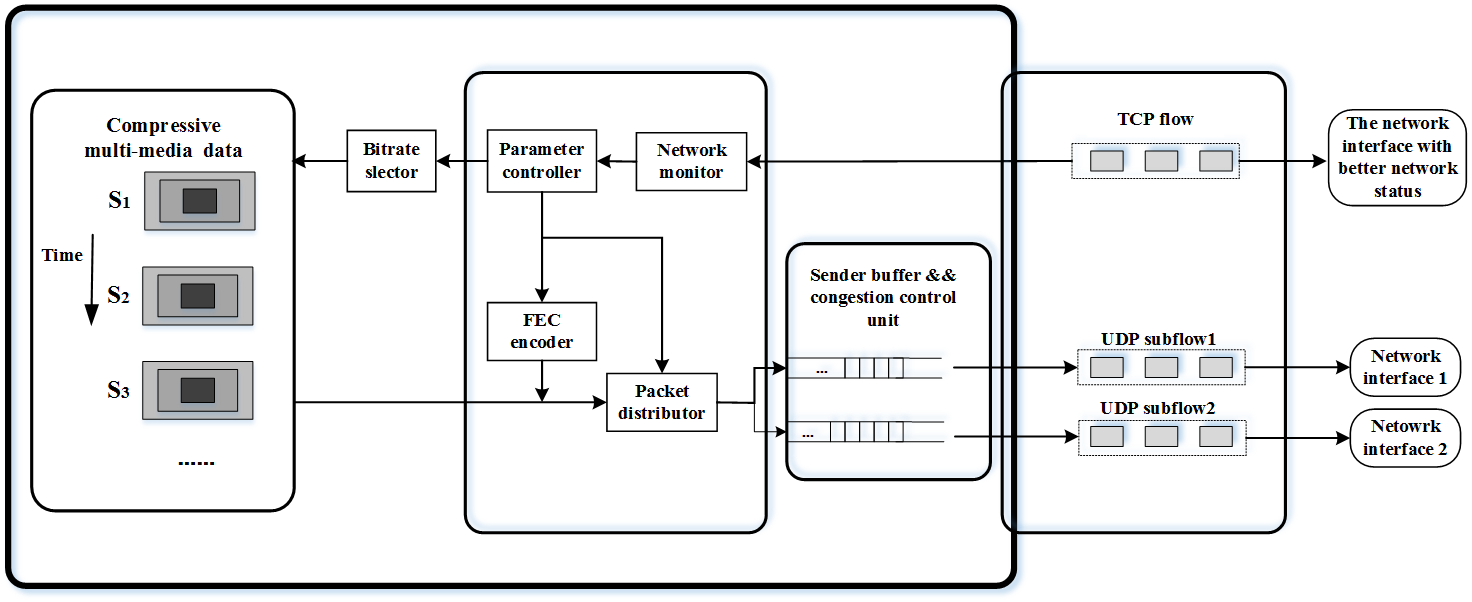
\includegraphics[scale=0.4]{paper_figs/architecture_V2.png}
	\caption{The Architecture of Protocol}
	\label{paper_figs:pathdemo}
\end{figure*}



%*****Instantaneous PSNR In relatively Bad Network Condition*****	

\begin{figure*}[!t]
	%\begin{figure*}[t]
	\centering
	\subfigure[Video Sequence 1]  {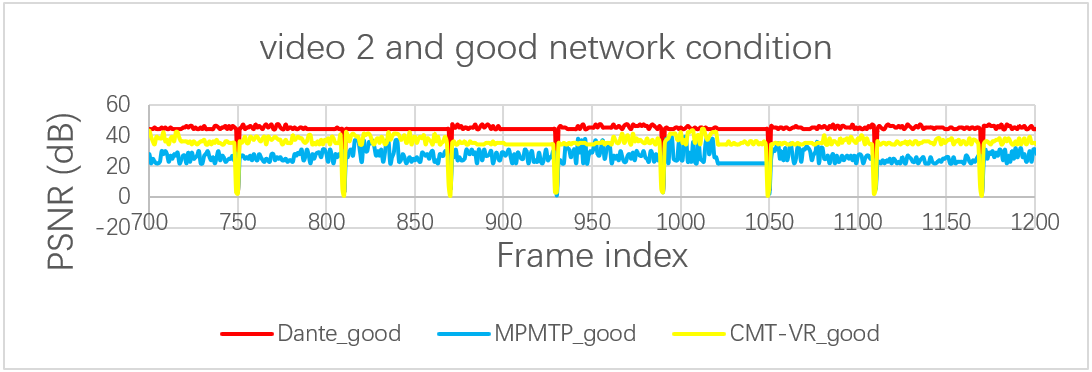
\includegraphics[scale=0.26,angle=0]{paper_figs/evaluation_result/sub/ins_psnr_v2_good.png}}
	\subfigure[Video Sequence 2]  {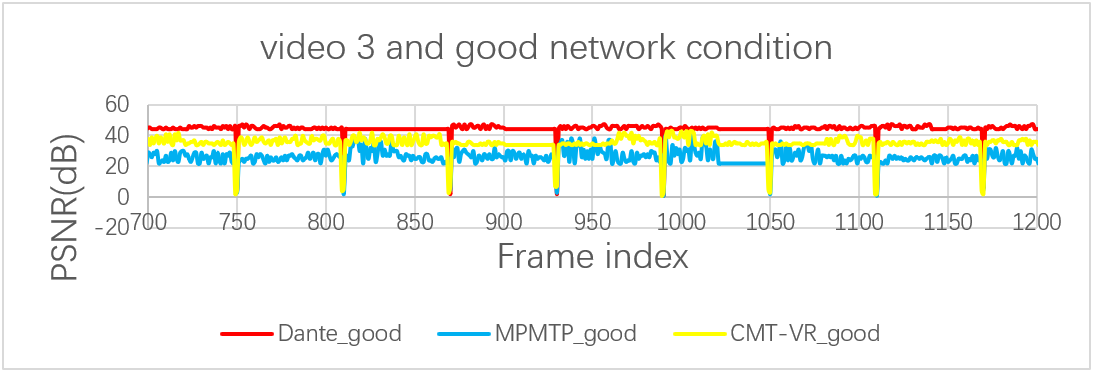
\includegraphics[scale=0.26,angle=0]{paper_figs/evaluation_result/sub/ins_psnr_v3_good.png}}
	\vspace{-0.3cm}
	\caption{Instantaneous PSNR In Relatively Good Network Condition}
	\vspace{-0.4cm}
	\label{fig:apuct}
\end{figure*}

%*****Instantaneous PSNR In relatively Good Network Condition*****
\begin{figure*}[!t]
	%\begin{figure*}[t]
	\centering
	\subfigure[Video Sequence 1]  {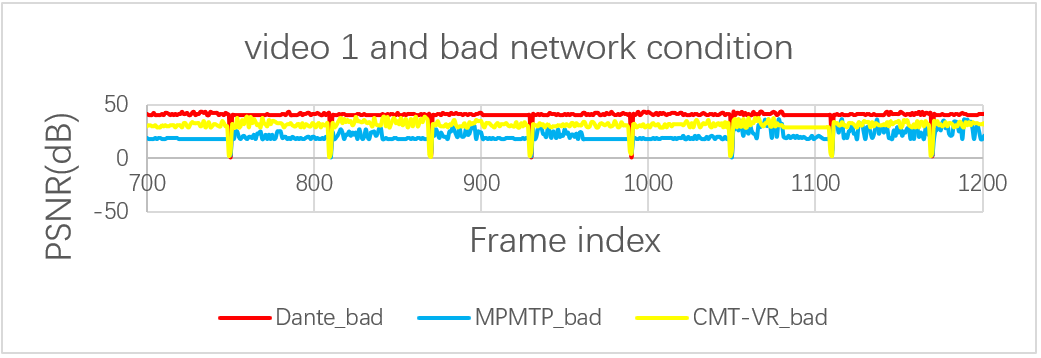
\includegraphics[scale=0.275,angle=0]{paper_figs/evaluation_result/sub/ins_psnr_v1_bad.png}}
	\subfigure[Video Sequence 2]  {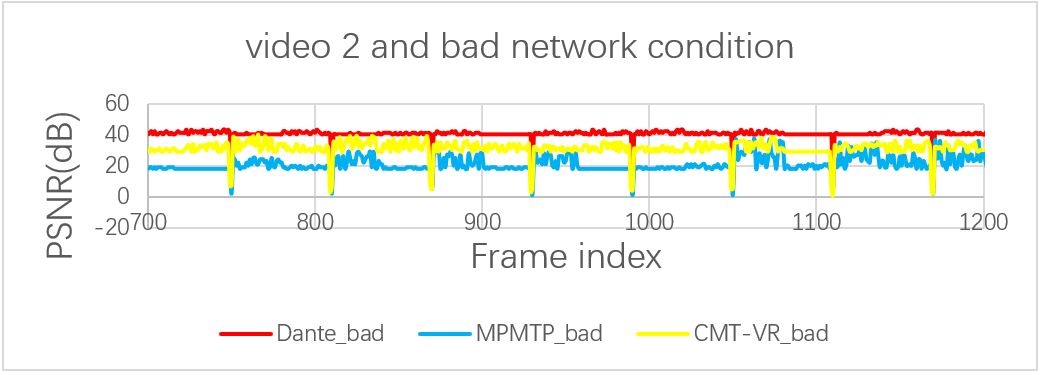
\includegraphics[scale=0.27,angle=0]{paper_figs/evaluation_result/sub/ins_psnr_v2_bad.png}}
	\vspace{-0.3cm}
	\caption{Instantaneous PSNR In Relatively Bad Network Condition}
	\vspace{-0.4cm}
	\label{fig:apuct}
\end{figure*}	




\section{Performance Evaluation}
We use PSNR as the metric of video quality and conducted extensive experiments to demonstrate Dante performance gains on video quality. 

\subsection{Reference schemes}
We evaluate the performance of Dante to compare with two video transport schemes, MPMTP~\cite{MPMTP} and CMT-VR~\cite{CMT-VR}, both of which are not FOV-aware and also utilize FEC to mitigating unnecessary retransmissions. Meanwhile, since the multi-path parallel is not our fous, so we do not take into account these two schemes' path selecting. 
\begin{packeditemize}

\item {\em MPMTP\cite{MPMTP}:} .
This video protocol utilizes the FEC to recover the data,  completely abandoning the retransmission,  in order to maximize the received data rate to prevent playback buffer starvation. This scheme performs in a video content-agnostic fashion. 

% high bandwidth
\item {\em CMT-VR\cite{CMT-VR}:}
CMT-VR, based on SCTP, utilize a quality-driven FEC redundancy  allocation to minimize the distortion of each GOP. Raptor code used to mitigate retransmission. While this scheme considers frame priority, \ie I, P frames, it is in a non-FOV-aware fashion. 

\end{packeditemize}


\subsection{Experimental Set-up}
\textbf{Experiment topology:} The server is connected with the client through one lossy links and Dante is deployed on both server and client side. The topology is not shown because of space limitation. The experiment scenario is that sources send the data to sinks through one lossy links with the request of video data.

\textbf{Testbed configuration:} The sources and sinks are commodity servers with Ubuntu 16.4 (kernel 4.40), each of which is equipped with an Intel(R) Core(TM) i3-4150k cpu @ 3.5GHz (4 cores), one Intel 82599ES 10G dual port NICs and 32 G memory.

\textbf{Parameter sets}
Timeout for triggering I frames' retransmission, $T_I$, is set to 200ms, the size of GOP is set to 15 and the length of video segment, which is request by users each time, is sent to 1s, equal to the time of 2 GOPs. Meanwhile, the size of the receiver buffer is set to 100Mb.
We evaluate the quality of video by computing the expected value of PSNR. So, given a video segment, it's PSNR can be calculated via: \[{V_{PSNR}} = \sum\limits_{i = 1}^{{\Omega ^\alpha }} {({\gamma ^\alpha } \cdot V_{PSNR}^{^\alpha })} \]
where, ${V_{PSNR}^{^\alpha }}$ is the PSNR of the layer $\alpha$. According to a tiles viewing probabilities \cite{360ProbDASH} and (Eq. 7), $\gamma ^\alpha$ can be approximately obtained and $\gamma ^\alpha$ of FOV layer, cushion layer and outmost layer is almost 0.6, 0.3, 0.1, respectively.

\textbf{Network parameter set:} Gilbert model is adopted to mimic the packet loss pattern in real wireless networks, supported by traffic control (TC)~\cite{TC}, in which four parameters($\xi _i^G$, $\xi _i^B$, 1-h and 1-k) are needed, $\xi _i^G$ and $\xi _i^B$ are transition probabilities between the bad and good state, 1-h and 1-k is the loss probability in the bad state and good state, respectively. In our testbed, 1-h and 1-k are set as 1 and 0, respectively. Meanwhile, average packet loss rate is equal to $\pi _i^B = \xi _i^B/(\xi _i^B\\ + \xi _i^P)$. And the bandwidth is also set by TC. The detailed Parameter set is seen in Table 2. 

\begin{table}
	\centering 
	\scriptsize
	\begin{tabular}{cp{1.0cm}p{1.6cm}p{0.8cm}p{2.3cm}}
		\rowcolor[gray]{0.9} 
		\hline
		(A)  &  Time(Sec.)    & Bandwidth(Mbps)       &  RTT(ms) &  Average Pakcet loss rate(\%) \\

		
		&  0${\sim}$60   &  30         &    50    &  0.5 \\

		\hline
		\rowcolor[gray]{0.9}
		\hline
		(B)  &   Time(Sec.)   & Bandwidth(Mbps)       &  RTT(ms) &     Average Pakcet loss rate(\%)  \\
		
		&  0${\sim}$60   &  20         &    50    &  2.5\\
		
		\hline
		
	\end{tabular}
	\caption{Network Condition of Two Wireless networks: (A)Relatively Good Wireless Conditions And (B)Relatively Bad Wireless Conditions}
	\label{}
\end{table}
`
\subsection{Performance Comparison With Existing Protocols}

Then, Figure 5 and Figure 6 compare instantaneous PSNR of three video sequences in good network condition and bad network condition, respectively. The result shows that Dante achieves 20\% to 30\% 360-degree video PSNR performance gain, compared to MPMTP and CMT-VR. The reason why MPMTP performs worst in all protocols is that, despite no involving retransmissions and maximizing the throughput, it doesn't consider video's inherent feature, such as decoding dependencies of video codec, which should have give different frame unequal attention, and thus can't utilize effectively the network allocation to boost video quality. Meanwhile, CMT-VR performs better than MPMTP, due to its consideration of frame priority. However, unfortunately, non-FOV-aware reliability scheme makes it waste valuable bandwidth on trivial data, thus CMT-VR is the secondary one. Dante takes into account not only traditional video features aforementioned, but FOV. Benefiting from the hierarchical protection spatially and temporally, Dante achieves desirable upgrade in instantaneous PSNR. Meanwhile, we find, compared to TCP without FEC, the average CPU time of Dante's, due to the introduction of FEC computing overhead, increases from 14\% to 25\% for the sender side, and from 14\% to 26\% for the receiver side. The overhead of FEC can be ignored considering the performance gain Dante achieves.      


\section{Conclusion}
In this paper, we propose a multipath protocol for 360-degree videos, which, based on multipath and FEC, performs hierarchical protection to counter limited bandwidth and error-prone problems in wireless networks. Experiments demonstrate Dante achieves desirable gains on 360-degree video QoE against reference schemes.  

\section*{ACKNOWLEDGEMENT}
The work was supported by the National Key Basic Research Program of China (973 program) under Grant 2014CB347800, National Key Research and Development Program of China under Grant 2016YFB1000200 and the National Natural Science Foundation of China under Grant No. 61522205, No. 61772305, No. 61432002. Dan Li is the corresponding author of this paper.

\bibliographystyle{abbrv}
\begin{small}
	\bibliography{apnet18}
\end{small}
\label{last-page}

\end{document}






\begin{figure}[ht]
	\centering
	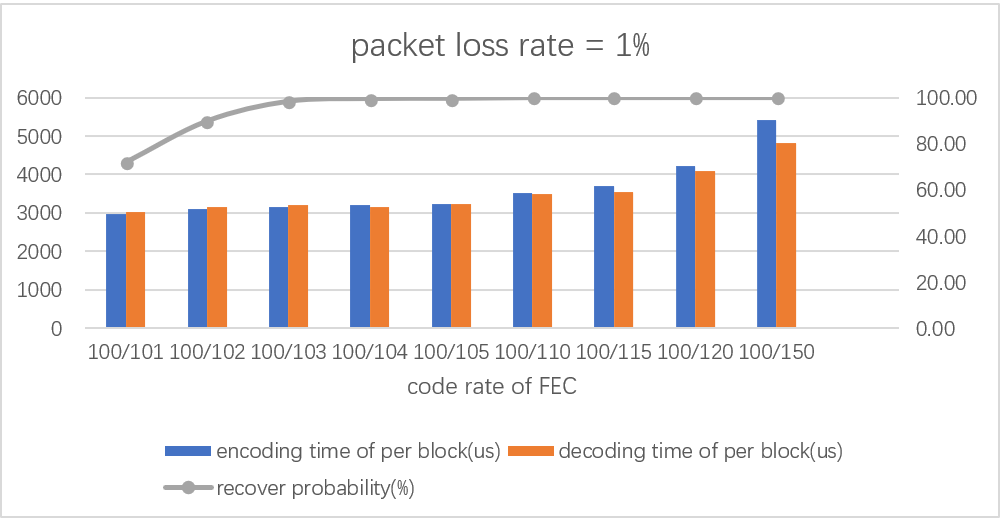
\includegraphics[scale=0.2]{paper_figs/RS_tradeoff.png}
	\caption{Tradeoff between recoverability and goodput}
	\label{paper_figs:pathdemo}
\end{figure}	 

\begin{figure}[ht]
	\centering
	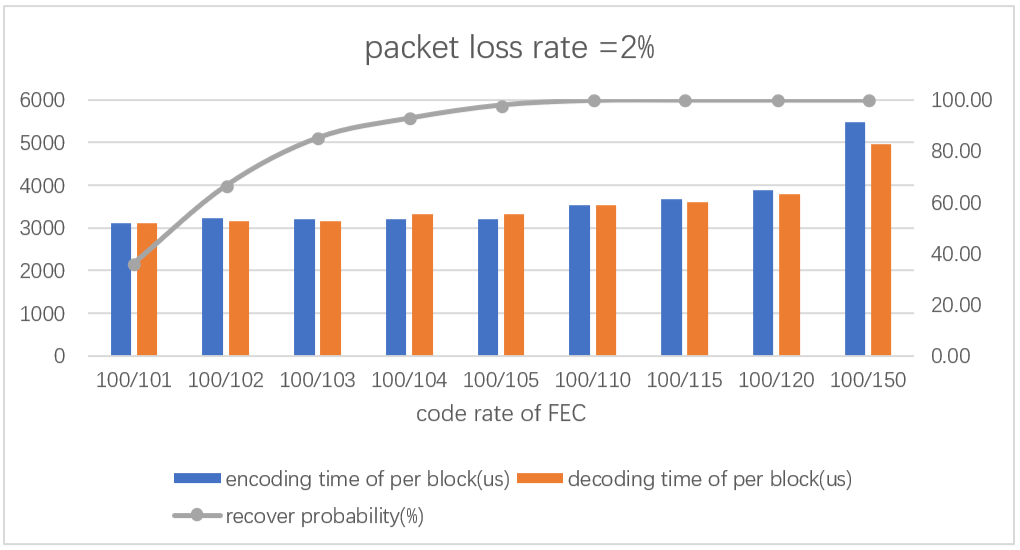
\includegraphics[scale=0.2]{paper_figs/RS_tradeoff_a.png}
	\caption{Tradeoff between recoverability and goodput}
	\label{paper_figs:pathdemo}
\end{figure}	




\begin{table*}
	\centering 
	\scriptsize
	\begin{tabular}{||p{1.35cm}<{\centering}||p{1.5cm}<{\centering}||p{1.7cm}<{\centering}
			||p{1.65cm}<{\centering} ||p{0.85cm}<{\centering} ||p{2.65cm}<{\centering}
			||p{2.0cm}<{\centering} || p{0.85cm}<{\centering} || p{0.85cm}<{\centering}||}
		\hline
		\rowcolor[gray]{0.9}
		\hline
		Solution & protocol layer   & video distortion model & data recovery& adaptive FEC & FEC parameter decision& data
		allocation&video-awareness& FOV-awareness\\
		\hline
		\hline
		MPLOT\cite{MPLOT} & transport layer & $\times$ & RS codes \& retransmissions & \checkmark
		& balance between goodput and recovery probability & packet generation's order & $\times$ & $\times$ \\
		\hline
		FMTCP\cite{FMTCP}    & transport layer  & $\times$ &Raptor codes \& retransmissions &
		\checkmark & balance between goodput and recovery probability & packet
		delivery time minimization & $\times$ & $\times$  \\
		\hline
		MPMTP\cite{MPMTP}  & application layer & $\times$ &Raptor codes & \checkmark & goodput maximization & block arrival time
		minimization & $\times$ & $\times$  \\
		\hline
		CMT-VR\cite{CMT-VR}   & transport layer & inflexible model & Raptor codes \&
		retransmissions & \checkmark & utility maximization& utility maximization &
		\checkmark & $\times$ \\
		\hline
		Dante    &application layer & proposed
		flexible model & RS code & \checkmark & hierarchical
		protection and distortion minimization & hierarchical protection & \checkmark & \checkmark \\
		\hline
	\end{tabular}
	\caption{MAIN DIFFERENCE OF THIS WORK WITH THE EXISTING WORKS}
	\label{}
\end{table*}
